\documentclass[11pt,a4paper]{article}
\usepackage[T1]{fontenc}
\usepackage{lmodern}
\usepackage[margin=25mm,headheight=15pt]{geometry}
\usepackage{amsmath,amssymb,amsthm,mathtools,bm}
\usepackage{booktabs,array,tabularx,longtable}
\usepackage{xcolor,microtype,enumitem,titlesec,fancyhdr}
\usepackage{tikz,pgfplots}
\usepackage{flafter}
\pgfplotsset{compat=1.18}
\usetikzlibrary{arrows.meta,positioning,calc}
\definecolor{ink}{HTML}{19334D}
\definecolor{accent}{HTML}{245E85}
\definecolor{curveone}{HTML}{1768AC}
\definecolor{curvetwo}{HTML}{D17B16}
\definecolor{curvethree}{HTML}{7B4DA6}
\usepackage[colorlinks=true,linkcolor=accent,urlcolor=accent,pdfauthor={},pdftitle={Fixed-Target CoreFalcon: An Explanatory Report},pdfsubject={Fixed-target norm rejection and conditional security},pdfcreator={pdfLaTeX}]{hyperref}
\pdfinfoomitdate=1
\pdftrailerid{}
\newcommand{\Z}{\mathbb Z}
\newcommand{\R}{\mathbb R}
\newcommand{\E}{\mathbb E}
\newcommand{\cL}{\Lambda}
\newcommand{\eps}{\varepsilon}
\newcommand{\norm}[1]{\left\lVert#1\right\rVert}
\newcommand{\abs}[1]{\left\lvert#1\right\rvert}
\newcommand{\rhoo}{\rho}
\newcommand{\TV}{\operatorname{TV}}
\newcommand{\chiq}{\chi^2}
\newcommand{\Adv}{\operatorname{Adv}}
\newcommand{\Var}{\operatorname{Var}}
\newcommand{\supp}{\operatorname{supp}}
\newcommand{\ind}{\mathbf 1}
\newtheorem{theorem}{Theorem}[section]
\newtheorem{lemma}[theorem]{Lemma}
\newtheorem{proposition}[theorem]{Proposition}
\newtheorem{corollary}[theorem]{Corollary}
\theoremstyle{definition}
\newtheorem{example}[theorem]{Example}
\newtheorem{definition}[theorem]{Definition}
\theoremstyle{remark}
\newtheorem{remark}[theorem]{Remark}
\setlength{\parindent}{0pt}
\setlength{\parskip}{5.5pt plus 1.5pt minus 1pt}
\setlength{\emergencystretch}{2em}
\widowpenalty=10000
\clubpenalty=10000
\displaywidowpenalty=10000
\linespread{1.035}
\setlist{topsep=4pt,itemsep=2pt,parsep=2pt,leftmargin=*}
\titleformat{\section}{\Large\bfseries\color{ink}}{\thesection}{0.65em}{}
\titleformat{\subsection}{\large\bfseries\color{ink}}{\thesubsection}{0.65em}{}
\titleformat{\subsubsection}{\normalsize\bfseries\color{ink}}{\thesubsubsection}{0.65em}{}
\titlespacing*{\section}{0pt}{18pt plus 3pt}{8pt}
\titlespacing*{\subsection}{0pt}{13pt plus 2pt}{5pt}
\pagestyle{fancy}
\fancyhf{}
\fancyhead[L]{\small\color{ink}Fixed-target CoreFalcon}
\fancyhead[R]{\small\color{ink}Explanatory report}
\fancyfoot[C]{\small\thepage}
\renewcommand{\headrulewidth}{0.3pt}
\numberwithin{equation}{section}
\setcounter{tocdepth}{1}
\begin{document}
{\LARGE\bfseries\color{ink}Fixed-Target CoreFalcon\par}
\vspace{4pt}
{\large An explanatory report\par}
\vspace{11pt}
\textbf{The question.} A lattice signer hashes a message with a fresh random salt, samples a candidate signature, and rejects candidates whose norm is too large. Can it retain that same salt and hash target while retrying, and still admit a concrete security proof?

\textbf{The answer in the declared model.} A discrete Gaussian with Falcon's original width remains sufficiently uniform across target cosets after the exact integer norm cutoff. At the two parameter sets, the acceptance-probability variance is below $2^{-90}$ and $2^{-120}$, and the accepted public image has chi-square distance below $2^{-81}$ and $2^{-83}$ from uniform. These analytical inequalities, evaluated with rigorous numerical enclosures, provide the missing distributional input to a fixed-target CoreFalcon security reduction.

The reduction retains explicit assumptions about the key distribution and exact-arithmetic sampler, as well as the costs of random-oracle programming, forgery extraction, and simulation. The primary concrete application uses a classical random oracle. The quantum-oracle corollary carries additional quantitative costs. The report develops the mathematical objects before using them, follows the central estimates, and then assembles the security statement and its scope.

\vspace{4pt}
\tableofcontents
\clearpage


\section{Why a retry policy becomes a security question}
\label{sec:retry-question}

A digital signature lets a recipient check that a message was approved by
someone holding a secret key. Producing the signature should require that
secret, while checking it should require only the corresponding public key.
In the lattice signature studied here, the signer must find a short integer
vector satisfying a public equation. Its secret key makes a suitable sampling
procedure efficient. A verifier checks the equation and the vector's length.

Sampling does not always produce a short enough vector. The signer therefore
rejects an unsuccessful sample and tries again. The question is what remains
fixed between attempts. It can keep the original equation and sample another
solution, or change the equation's target before resampling. Both procedures
can return perfectly valid signatures. Nevertheless, their output distributions
need not agree, and a security argument for one procedure need not prove
security of the other.

Suppose two targets are initially equally likely. At target~0 a proposed
solution passes with probability $1/2$; at target~1 it always passes. If the
target is chosen once and retained, target~0 merely takes longer to finish.
The final target probabilities remain $(1/2,1/2)$. If every failed attempt
restarts with a new uniform target, the successful masses in one attempt are
$(1/4,1/2)$. Normalizing gives final probabilities $(1/3,2/3)$. The second
procedure favors the easier target.

This distinction matters because a security proof often answers signing
requests through a simulator that has no secret key. Rather than solve a
chosen equation, the simulator can sample a short vector first and calculate
which target it solves. It then arranges the modeled hash value to equal that
target. For this strategy to be useful, its joint distribution of targets and
vectors must be sufficiently close to the real signer's distribution. Returning
valid vectors alone is insufficient.

The central result controls this distributional comparison after Falcon's norm
test. It applies at the original parameters, uniformly over keys satisfying
the stated geometric promises. The resulting security statement concerns the
mathematical CoreFalcon model: a fresh initial salt, one target per signing
request, and private retries at that target. The proof has an analytic part,
which studies a norm-conditioned integer Gaussian, and a cryptographic part,
which converts that estimate into a simulation and forgery reduction. We first
identify exactly which probability laws these two parts must connect.

\section{The public equation and its Gaussian solutions}
\label{sec:equation-gaussian}

\subsection{A target selects a set of integer vectors}

Fix $q=12289$ and $n\in\{512,1024\}$. A ring element is represented by a
polynomial of degree less than $n$. Multiplication is performed with the rule
$X^n=-1$. The integer-coefficient ring and its finite reduction modulo $q$ are
\[
 \mathcal R=\Z[X]/(X^n+1),
 \qquad \mathcal R_q=\mathcal R/q\mathcal R.
\]
The public key is $h\in\mathcal R_q$. A proposed solution is a pair
$z=(u,v)\in\mathcal R^2$, with public target, or \emph{syndrome},
\[
 F_h(u,v)=u+hv\pmod q.
\]
Writing the coefficients of $u$ and $v$ consecutively identifies $z$ with a
vector in $\Z^d$, where $d=2n$. Its squared norm is the sum of the squares of
all $2n$ coefficients. Every norm of a signature vector uses this coefficient
representation.

The solutions of $F_h(z)=0$ form a lattice
$\Lambda_h\subset\Z^d$: a discrete additive set closed under integer linear
combinations. If $z_y$ is one solution of $F_h(z)=y$, all solutions at that
target are precisely
\[
 F_h^{-1}(y)=z_y+\Lambda_h.
\]
Such a translated lattice is called a \emph{coset}. Subtracting two solutions
at the same target gives a lattice vector; adding a lattice vector to one
solution gives another. A target therefore specifies a whole collection of
possible vectors, not a unique answer.

The map is onto: for any $y$, the pair $(u,v)=(y,0)$ is a solution modulo
$q$. This does not usually give a short enough solution to sign. There are
$q^n$ different targets, so the quotient
\[
 Y=\Z^d/\Lambda_h
\]
has cardinality $|Y|=q^n$ and can be identified with $\mathcal R_q$.
This algebraic fact holds for every public $h$; it does not require $h$ to be
invertible. Let $U(y)=1/|Y|$ denote the uniform target law.

\subsection{A discrete Gaussian and its conditional law}

A Gaussian on integer vectors assigns greater probability to shorter vectors.
For width $\sigma>0$, define
\[
 G(z)=\frac{\exp(-\norm{z}^2/(2\sigma^2))}
 {\displaystyle\sum_{x\in\Z^d}\exp(-\norm{x}^2/(2\sigma^2))}.
\]
The denominator normalizes the positive masses to sum to one. This is an
integer distribution, even though its weights use the familiar Gaussian
exponential. The width specifies the exponent; the variance of a discrete
coordinate is not defined to equal $\sigma^2$.

Let
\[
 \mu(y)=\Pr_{Z\leftarrow G}[F_h(Z)=y],
 \qquad
 G_y(z)=\frac{G(z)}{\mu(y)}\,\mathbf{1}[F_h(z)=y].
\]
Here $G_y$ is the Gaussian restricted to the solutions at target $y$ and
renormalized. The public experiment draws $Z$ from $G$ and then computes
$F_h(Z)$. A reverse experiment first chooses $y$ and then draws from $G_y$.
If the reverse experiment chooses $y$ according to $\mu$, their joint laws
agree exactly. If it chooses a uniform $y$, the agreement depends on how close
$\mu$ is to uniform.

This is the role of Gaussian \emph{smoothing}: at a sufficiently large width,
the total Gaussian masses of different lattice cosets become nearly equal.
The secret basis supplies a geometric bound that makes the smoothing
estimate uniform over permitted keys.
The next part of the report establishes that geometric input. Smoothing before
any rejection, however, is only a starting point. Restricting to short vectors
can favor some targets over others.

\section{What the signer does and what the verifier sees}
\label{sec:signing-experiment}

The accepted event is
\[
 A=\{z:\norm{z}^2\le T\}.
\]
Because squared norms of integer vectors are integers, rejection starts at
the exact boundary $K=T+1$.

\begin{samepage}
The relevant parameters are
\begin{center}
\begin{tabular}{lrr}
\toprule
 & Degree 512 & Degree 1024\\
\midrule
Coefficient dimension $d$ & 1024 & 2048\\
Gaussian width $\sigma$ (approximately) & 165.736617 & 168.388571\\
Largest accepted squared norm $T$ & 34,034,726 & 70,265,242\\
First rejected squared norm $K$ & 34,034,727 & 70,265,243\\
Salt length $\kappa$ & 320 bits & 320 bits\\
\bottomrule
\end{tabular}
\end{center}
\end{samepage}
The exact width formula will be given with the geometric and numerical
estimates. Rounded decimals are descriptive rather than definitions.

The hash is modeled as a random oracle
\[
 H:\mathsf{PK}\times\{0,1\}^{\kappa}\times\mathsf{Msg}
 \longrightarrow\mathcal R_q.
\]
This means that distinct inputs have independent uniform outputs, while
repeating an input returns its previously assigned value. The tuple contains
the public key, salt and message with an unambiguous encoding. The model
concerns one honestly generated key. Let $\mathsf{Gen}$ denote its specified
exact mathematical NTRU trapdoor-generation distribution. It supplies the
public key, secret basis, and FFO sampling tree; the geometric and sampler
contracts below hold for every key in its support. Random-oracle programming
is a proof operation in this ideal hash model.

For a message $m$, the signer draws an independent uniform salt $r$ after
receiving the message and sets $y=H(h,r,m)$. It then repeatedly draws
$(u,v)$ from its secret-key sampling distribution $P_y$, using fresh private
coins, until $A$ holds. Throughout this loop it retains both $r$ and $y$.
It returns the mathematical signature $(r,v)$.

The declared exact-arithmetic fast-Fourier orthogonalization (FFO) sampler
has law $P_y$, which need not equal the exact coset-Gaussian law $G_y$. Its proved probability-ratio profile
enters the security comparison in Section~\ref{sec:tree-sampler};
Section~\ref{sec:key-quality} checks the geometric hypotheses needed there.

Verification recomputes $y$ and reconstructs
\[
 \widehat u=\operatorname{ctr}_q(y-hv),
\]
where $\operatorname{ctr}_q$ reduces every coefficient to an integer in
$[-6144,6144]$. It accepts the mathematical signature when
$\norm{(\widehat u,v)}^2\le T$. Centering cannot increase any coefficient's
absolute value, so an accepted sampled pair always yields a valid signature.
The sampled $u$ can differ from $\widehat u$, especially at degree 1024.
The probability comparison therefore studies the sampled pair before this
public reconstruction.

Only the final signature, or a specified public error, is revealed. Retry
counts, intermediate vectors and running times are absent from the interface.
Messages may be chosen adaptively using previous answers. Signing requests
remain classical even in the quantum-oracle variant; quantum access concerns
the hash queries. The security proof bounds the probability that the fresh salt selects a
previously queried signing input before replacing its target by a fresh
uniform one.

These conditions define the signing interface used below.
Section~\ref{sec:representation} treats the canonical compressed wrapper,
and Section~\ref{sec:model-boundary} collects changes requiring further analysis.

\section{Three distributions of accepted targets}
\label{sec:three-laws}

Write
\[
 a_y=\Pr_{Z\leftarrow G_y}[A],
 \qquad
 \delta=\Pr_{Z\leftarrow G}[A^c].
\]
The first number depends on the target; the second averages rejection under
the ambient Gaussian. Assume for now that every $a_y$ is positive, as the
later uniform rejection bound will establish.

\subsection{Choose a uniform target and keep it}

In the ideal uniform-target experiment, choose $y\leftarrow U$ once and
repeat independent $G_y$ draws until acceptance. The accepted vector law at
that target is $G_y\mid A$. Indeed, the probability of eventually returning
a particular accepted vector $z$ is
\[
 \sum_{j=0}^{\infty}(1-a_y)^jG_y(z)
 =\frac{G_y(z)}{a_y}.
\]
Every chosen target eventually succeeds, so its marginal law remains $U$.
In the proof experiment where each signing request receives a fresh uniform
target, the real sampler analog is the joint law
\[
 L(y,z)=U(y)P_y(z\mid A).
\]
The norm theorem first addresses the ideal Gaussian; the sampler comparison
then returns to this real accepted law.

\subsection{Choose a new uniform target after each failure}

Suppose instead that each attempt chooses a new uniform target and one
$G_y$ sample. The successful target masses per attempt are $U(y)a_y$.
The final target law is therefore
\[
 \widetilde\nu(y)=\frac{U(y)a_y}{\E_{y\leftarrow U}a_y}.
\]
Targets with higher acceptance probability appear more often. This experiment weights only the acceptance probabilities. The public
simulator below also weights the original Gaussian image.

\subsection{Accept an ambient Gaussian and compute its target}

The public simulator draws from $G$ until the norm test succeeds and then
computes the syndrome. It knows no trapdoor. The probability that one ambient
draw both has target $y$ and passes is $\mu(y)a_y$. Hence its accepted
target law and joint law are
\[
 \nu(y)=\frac{\mu(y)a_y}{1-\delta},
 \qquad
 M(y,z)=\nu(y)G_y(z\mid A).
\]
Equivalently, $M$ samples $z\leftarrow G\mid A$ and sets $y=F_h(z)$.
The conditional ideal vector law agrees with fixed-target signing, but the
target weights differ. Both the unconditioned image $\mu(y)$ and the
acceptance factor $a_y$ must be controlled.

\subsection{A finite example showing all three laws}

Consider a public proposal with three possible outcomes:
\begin{center}
\begin{tabular}{llcr}
\toprule
Outcome & Target & Passes? & Probability\\
\midrule
$z_0^+$ & 0 & Yes & $3/8$\\
$z_0^-$ & 0 & No  & $3/8$\\
$z_1^+$ & 1 & Yes & $1/4$\\
\bottomrule
\end{tabular}
\end{center}
Its target distribution is $\mu=(3/4,1/4)$, while the conditional
acceptance probabilities are $(a_0,a_1)=(1/2,1)$. Keeping an initially uniform
target produces $(1/2,1/2)$. Redrawing a uniform target produces
\[
 \widetilde\nu=\frac{(1/4,1/2)}{3/4}=(1/3,2/3).
\]
Accepting the public proposal produces
\[
 \nu=\frac{(3/8,1/4)}{5/8}=(3/5,2/5).
\]
All procedures return a passing outcome, yet all three target laws differ.
The distinction also changes expected attempt counts: respectively $3/2$,
$4/3$ and $8/5$. These are illustrative probability calculations, not small
Falcon instances or speed estimates.

\begin{figure}[htbp]
\centering
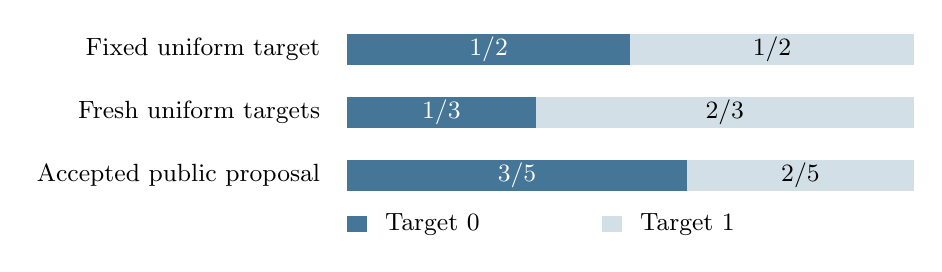
\begin{tikzpicture}[x=7.2cm,y=0.8cm,font=\small]
 \fill[accent!85] (0,2) rectangle (0.5,2.5);
 \fill[accent!20] (0.5,2) rectangle (1,2.5);
 \fill[accent!85] (0,1) rectangle ({1/3},1.5);
 \fill[accent!20] ({1/3},1) rectangle (1,1.5);
 \fill[accent!85] (0,0) rectangle (0.6,0.5);
 \fill[accent!20] (0.6,0) rectangle (1,0.5);
 \node[anchor=east] at (-0.03,2.25) {Fixed uniform target};
 \node[anchor=east] at (-0.03,1.25) {Fresh uniform targets};
 \node[anchor=east] at (-0.03,0.25) {Accepted public proposal};
 \node[text=white] at (0.25,2.25) {$1/2$};
 \node at (0.75,2.25) {$1/2$};
 \node[text=white] at ({1/6},1.25) {$1/3$};
 \node at ({2/3},1.25) {$2/3$};
 \node[text=white] at (0.3,0.25) {$3/5$};
 \node at (0.8,0.25) {$2/5$};
 \fill[accent!85] (0,-0.65) rectangle (0.035,-0.4);
 \node[anchor=west] at (0.05,-0.525) {Target 0};
 \fill[accent!20] (0.45,-0.65) rectangle (0.485,-0.4);
 \node[anchor=west] at (0.50,-0.525) {Target 1};
\end{tikzpicture}
\caption{The three accepted target laws in the finite example. Every row is a probability distribution summing to one. The public proposal has target weights $(3/4,1/4)$ before acceptance; the two target acceptance probabilities are $(1/2,1)$.}
\label{fig:three-laws}
\end{figure}

The mathematical task can now be stated precisely. Ordinary smoothing
controls the ambient target weights. The new norm-tail analysis must control
the effect of keeping only short vectors. Together, these estimates must make
the accepted public law sufficiently close to uniform-target fixed retries,
in the direction needed by the security reduction. A small average bias alone
will not be the entire argument: the proof must also rule out accepted targets
with dangerously tiny probability and include the actual sampler error.


\section{Controlling a sharp integer norm cutoff}
\label{sec:norm}

We now bound the accepted ambient image just identified, uniformly over the
permitted keys. The proof separates ordinary Gaussian smoothing from the
additional bias introduced by the integer norm cutoff.

\subsection{The precise geometric statement}

Let $n$ be either $512$ or $1024$, let $d=2n$, and set
$q=12289$ and $B_0=(117/100)\sqrt q$. Consider any full-rank sublattice
$\Lambda\subset\Z^d$ of index $N=q^n$ that has a basis whose
Gram--Schmidt lengths are all at most $B_0$. The index is the number of
cosets: the quotient group $Y=\Z^d/\Lambda$ has $N$ elements. The bounds
hold for every lattice in this class.

An ordered basis $b_1,\ldots,b_d$ generates the lattice by integer linear combinations. Its Gram--Schmidt vector $\widetilde b_i$ is the part of $b_i$ orthogonal to the real span of the preceding basis vectors. Bounding these orthogonal lengths controls Gaussian sums even if the original basis vectors themselves are longer.

Write $X\sim G$ for an ambient Gaussian vector, in product form:
\begin{equation}
 \Pr[X=x]=\frac{e^{-\alpha\norm{x}^2}}{Z_\alpha^d},
 \qquad \alpha=\frac1{2\sigma^2},\qquad
 Z_\alpha=\sum_{j\in\Z}e^{-\alpha j^2}.
 \label{eq:norm-gaussian}
\end{equation}
The coordinates are independent before conditioning and are dimensionless
integers. The admissible parameters
are the following exact decimal intervals and integer cutoffs.

\begin{center}
\small
\begin{tabular}{@{}r r l r@{}}
\toprule
$n$ & $d$ & Width interval for $\sigma$ & $T$\\
\midrule
512 & 1024 & $[165.736617182977,\,165.736617182979]$ & 34034726\\
1024 & 2048 & $[168.388571446543,\,168.388571446545]$ & 70265242\\
\bottomrule
\end{tabular}
\end{center}

For a coset $y\in Y$, define its acceptance probability by
\[
 a_y=\Pr[\norm X^2\le T\mid X\bmod\Lambda=y].
\]
Let $U$ be uniform on $Y$, and let $\nu$ be the law of
$X\bmod\Lambda$ conditional on $\norm X^2\le T$. For every lattice and
every width in the corresponding interval, the result is
\begin{equation}
\begin{array}{c|cc}
 & n=512 & n=1024\\\hline
\operatorname{Var}_{y\sim U}(a_y)&<2^{-90}&<2^{-120}\\
\chi^2(\nu\Vert U)&<2^{-81}&<2^{-83}.
\end{array}
\label{eq:norm-main}
\end{equation}
Here variance measures variation over uniformly chosen targets, and
$\chi^2(\nu\Vert U)=\E_U[(d\nu/dU-1)^2]$ measures the mean squared
departure of the accepted syndrome density from one. Neither statement
identifies the overall rejection probability with these tiny numbers.
The same bounds remain valid if acceptance also requires
$|X_j|\le2047$ on any fixed set of $n$ coordinates.

\subsection{Why the key-quality check supplies the basis hypothesis}
\label{sec:key-quality}

The public map is $F_h(s_1,s_2)=s_1+hs_2\pmod q$, with
$h=g/f\pmod q$ in $\Z_q[X]/(X^n+1)$ and $f$ invertible modulo $q$.
The secret polynomials satisfy $fG-gF=q$. Since the first component of
$F_h$ has coefficient one, the map is onto and
$\Lambda_h=\ker F_h$ has index $q^n$.

Expand the two polynomial columns
$u_1=(g,-f)$ and $u_2=(G,-F)$ into all their negacyclic coefficient
shifts, placing the first block before the second. Their coefficient
determinant has absolute value $q^n$, so they generate exactly
$\Lambda_h$. A negacyclic shift rotates coefficients with a possible
sign change and preserves Euclidean length.

Write $a^*=a(X^{-1})$ in the quotient ring and $D=ff^*+gg^*$.
The fractions below are computed in the real coefficient algebra
$\R[X]/(X^n+1)$. At a complex root $\zeta$ of $X^n+1$,
$D(\zeta)=|f(\zeta)|^2+|g(\zeta)|^2>0$: the equation $fG-gF=q$
prevents $f$ and $g$ from vanishing together. Thus $D$ is invertible.
The mathematical key-generation check is
\[
 \max\left\{\norm{(g,-f)},
 \left\|\left(\frac{qf^*}{D},\frac{qg^*}{D}\right)\right\|\right\}
 \le B_0.
\]
This initially bounds two polynomial vectors. To see why it bounds
every ordinary Gram--Schmidt length, let $W$ be the real span of the
shifts of $u_1$. Orthogonal projection cannot increase a length, so all
first-block Gram--Schmidt vectors have length at most $\norm{u_1}$.
For the second block, the identity
\[
 u_2-\frac{Gg^*+Ff^*}{D}u_1
   =v:=\left(\frac{qf^*}{D},\frac{qg^*}{D}\right)
\]
exhibits the projection onto $W^\perp$: the polynomial inner product of
$u_1$ and $v$ vanishes, and therefore $v$ is orthogonal to every shift
of $u_1$. Shifts preserve $W$ and its orthogonal complement. Each
second-block vector first projects to a shift of $v$; further
Gram--Schmidt projections can only shorten it. Hence every resulting
length is at most $B_0$. The argument permits any ordering within a block.

Splitting a polynomial as $a(X)=a_{\rm even}(X^2)+X a_{\rm odd}(X^2)$ merely rearranges its coefficients into the even and odd positions, preserving their total squared norm. Repeating this split expands the sampling tree into ordinary coefficient coordinates. The exact tree factorization identifies the sampler's
unnormalized leaf values $D_i$ with these squared lengths. Thus
$\sqrt{D_i}\le B_0$ and its one-dimensional widths satisfy
$\sigma_i=\sigma/\sqrt{D_i}\ge\sigma/B_0$. This establishes the geometric
input to the exact-arithmetic sampler profile. The exact-arithmetic profile is used in Section~\ref{sec:tree-sampler}.

The exact parameter definitions are
\[
\begin{aligned}
 \eps_{\mathrm{des}}&=(2^{64}\lambda)^{-1/2},\\
 \sigma&=\frac{B_0}{\pi}
 \sqrt{\frac{\ln(4n(1+1/\eps_{\mathrm{des}}))}{2}},\\
 T&=\left\lfloor\frac{121}{100}d\sigma^2\right\rfloor.
\end{aligned}
\]
Here $\ln$ is the natural logarithm, and $\lambda=128$ or $256$ is the
sampler design parameter at the respective degree. These exact widths lie
in the displayed intervals.

\subsection{Separate the original image from the rejected image}

Since squared norms are integers, rejection starts at $K=T+1$.
Introduce two densities relative to $U$:
\[
 p(y)=N\Pr[X\bmod\Lambda=y],\qquad
 r(y)=N\Pr[X\bmod\Lambda=y,\ \norm X^2\ge K].
\]
Their uniform means are $\E_U p=1$ and
$\E_U r=\delta=\Pr[\norm X^2\ge K]$. The conditional rejection
probability at a particular target is $\delta_y=r(y)/p(y)$, so
$a_y=1-\delta_y$. Positivity of every coset Gaussian mass makes this
division well-defined. The accepted image has the exact density
\begin{equation}
 \frac{d\nu}{dU}(y)=\frac{p(y)-r(y)}{1-\delta}.
 \label{eq:norm-accepted-density}
\end{equation}
The normalization in this formula is ambient acceptance, not the
uniform-target average of $a_y$.

The two centered norms to control are
\[
 Q_0=\bigl(\E_U|p-1|^2\bigr)^{1/2},\qquad
 R=\bigl(\E_U|r-\delta|^2\bigr)^{1/2}.
\]
Ordinary smoothing controls $Q_0$. The new difficulty is $R$, because
the indicator of a sharp integer norm cutoff does not factor into
independent coordinate weights.

For $c>0$, write $\rho_c(S)=\sum_{x\in S}e^{-c\norm x^2}$ and
$\vartheta(c)=\sum_{j\in\Z}e^{-cj^2}$. The dual lattice
$\Lambda^*=\{w:\langle w,\Lambda\rangle\subset\Z\}$ represents the
frequencies of the quotient: its characters are
$\widehat Y=\Lambda^*/\Z^d$. A character evaluates the phase
$e^{2\pi i\langle w,x\rangle}$ and is constant on each coset.
Finite Fourier orthogonality gives Parseval's identity
\begin{equation}
 R^2=\sum_{w\in\widehat Y\setminus\{0\}}
 \left|\E\!\left[e^{2\pi i\langle w,X\rangle}
       \mathbf1_{\{\norm X^2\ge K\}}\right]\right|^2.
 \label{eq:norm-parseval}
\end{equation}
The trivial character is omitted because $R$ is centered. The task is
to bound this whole sum, without multiplying a per-character bound by
the enormous number $N$.

\subsection{The smoothing estimates available before rejection}

The reversed dual basis has Gram--Schmidt lengths reciprocal to the
original ones, hence at least $1/B_0$. Summing its coefficients
successively gives
\[
 \rho_c(\Lambda^*)\le\vartheta(c/B_0^2)^d,
 \qquad \vartheta(c)\le1+\sqrt{\pi/c}.
\]
The first bound uses the fact that a shifted Gaussian sum is largest at
an unshifted lattice. Poisson summation explains that fact: its expression
for $\rho_c(L+z)$ has nonnegative Gaussian magnitudes multiplied by
phases, so replacing every phase by one bounds it by $\rho_c(L)$.

Define
$\eta_c=\vartheta(\pi^2/(cB_0^2))^d-1$. For clarity, the Poisson identity used here is
\[
 \rho_c(L+z)=\frac{(\pi/c)^{d/2}}{\det L}
 \sum_{w\in L^*}e^{-\pi^2\norm{w}^2/c}
 e^{2\pi i\langle w,z\rangle}.
\]
Here $\det L$ is the volume of a basis parallelepiped; it equals $N$ for a sublattice of $\Z^d$ of index $N$. The term $w=0$ gives the central, translate-independent mass. The absolute sum of all other terms bounds its possible variation. This identity converts the geometric dual-mass estimate into the probability estimate that follows.

The same dual expansion yields
\begin{equation}
 \frac{(\pi/c)^{d/2}}N(1-\eta_c)
 \le\rho_c(\Lambda+z)
 \le\frac{(\pi/c)^{d/2}}N(1+\eta_c)
 \label{eq:norm-flat-cosets}
\end{equation}
for every real translate $z$. In particular $|p(y)-1|\le\eta_\alpha$.
When deriving this last bound, the integer dual vectors contribute
phase one and must be canceled against the ambient normalization before
taking absolute values. Counting them as error would weaken the bound.

An energy estimate is sharper than this pointwise bound. Put
$A_0=\pi^2/\alpha$. For a frequency coset $C=\Z^d-w$ and
$0<\xi<2$, weighted Cauchy--Schwarz gives
$\rho_{A_0}(C)^2\le\rho_{\xi A_0}(C)\rho_{(2-\xi)A_0}(C)$.
Apply it to each frequency coset, bound the first factor by an
unshifted mass, and sum the second over the nontrivial characters. This gives
\begin{equation}
 Q_0^2\le\vartheta(\xi A_0)^d
 \left[\vartheta\!\left(\frac{(2-\xi)A_0}{B_0^2}\right)^d-1\right].
 \label{eq:norm-Q0}
\end{equation}
Let $\overline Q_0$ be the square root of the right-hand expression,
evaluated with the tuning parameter $\xi=1/100$. Its role is to split this
inequality; the sampler-width parameter $\eps_{\mathrm{des}}$ has a separate
definition.

\subsection{An exact integral for a discrete tail}

Set $\beta=d/(2K)$ and $t=\alpha-\beta>0$. The positive tilt $t$
separates a Gaussian decay factor from an exact selector of integer
norms. For $\operatorname{Re}z>0$, define the twisted theta sum
\[
 \Theta(z,u)=\sum_{x\in\Z}e^{-zx^2+2\pi iux}.
\]
For each character $w$, its rejected-tail coefficient is exactly
\begin{align}
 &\E\!\left[e^{2\pi i\langle w,X\rangle}
       \mathbf1_{\{\norm X^2\ge K\}}\right]\\
 &\quad=\frac{e^{-tK}}{2\pi Z_\alpha^d}
 \int_{-\pi}^{\pi}
 \frac{\prod_{j=1}^d\Theta(\beta-i\theta,w_j)
       e^{-iK\theta}}{1-e^{-t-i\theta}}\,d\theta.
 \label{eq:norm-contour}
\end{align}
To verify the selector, expand the denominator as
$\sum_{j\ge0}e^{-tj-ij\theta}$. A vector of squared norm $m$
contributes a phase $e^{i(m-K-j)\theta}$, whose integral vanishes unless
$j=m-K$. Such a nonnegative integer $j$ exists exactly when $m\ge K$.
The surviving weight is
$e^{-tK}e^{-\beta m}e^{-t(m-K)}=e^{-\alpha m}$, as required.
The positive $\beta,t$ give absolute convergence, justifying the
exchanges of integration and summation. This is an identity for the
integer Gaussian, rather than a continuous radial approximation.

Minkowski's inequality allows us to bound the Euclidean norm of the
vector of nontrivial coefficients by integrating its pointwise norm.
We therefore need good aggregate estimates at the different angles
$\theta$.

\subsection{Rational angles reveal the arithmetic cancellation}

Write $\theta=\pi a/b+v$ with $\gcd(a,b)=1$ and $b\ge1$. The integer
quadratic phase $\phi_{a,b}(x)=e^{i\pi ax^2/b}$ obeys
$\phi_{a,b}(x+b)=(-1)^{ab}\phi_{a,b}(x)$. Let $\eta_b=0$ when $ab$ is even and
$\eta_b=1/2$ when it is odd. A finite Fourier expansion then has the form
\[
 \phi_{a,b}(x)=\sum_{\ell=0}^{b-1}c_\ell
 e^{2\pi i(\ell+\eta_b)x/b},\qquad |c_\ell|=b^{-1/2}.
\]
The half-frequency is necessary in the antiperiodic case. The uniform
coefficient magnitude follows by autocorrelation: after removing the
half-frequency, the correlation at shift $h$ contains
$\sum_{x=0}^{b-1}e^{2\pi iahx/b}$, which vanishes unless $b$ divides
$h$. Fourier transforming this correlation gives
$|c_\ell|^2=1/b$.

Put $h_v=\sqrt{\beta^2+v^2}$ and
$A_v=\pi^2\beta/(\beta^2+v^2)$. The one-dimensional complex Poisson identity is
\[
 \Theta(z,u)=\sqrt{\frac\pi z}
 \sum_{k\in\Z}\exp\!\left(-\frac{\pi^2(k-u)^2}{z}\right),
 \qquad \operatorname{Re}z>0,\quad u\in\R.
\]
The square root is the branch positive on positive real $z$.
For $z=\beta-iv$, its prefactor has modulus $\sqrt{\pi/h_v}$
and $\operatorname{Re}(1/z)=\beta/h_v^2$. The $b$ shifted frequency sums
from the finite expansion merge into $b^{-1}(\Z+\eta_b)$.
Applying these facts in each coordinate gives
\begin{equation}
 \left|\prod_{j=1}^d\Theta(\beta-i\theta,w_j)\right|
 \le\left(\frac\pi{bh_v}\right)^{d/2}
 \rho_{A_v}\!\left(b^{-1}(\Z^d+\eta_b\mathbf1)-w\right).
 \label{eq:norm-rational}
\end{equation}
This converts oscillatory cancellation into a decaying Gaussian mass.

The decisive summation step uses the finite quotient. If $\gcd(b,N)=1$,
multiplication by $b$ permutes $\widehat Y$. Consequently
\begin{equation}
 \sum_{w\in\widehat Y}
 \rho_c\!\left(b^{-1}(\Z^d+\eta_b\mathbf1)-w\right)
 =\rho_{c/b^2}(\Lambda^*+\eta_b\mathbf1).
 \label{eq:norm-merger}
\end{equation}
Indeed, multiplying every summation vector by $b$ produces the sets
$\Z^d+\eta_b\mathbf1-bw$. They form a disjoint decomposition of the
translated dual lattice. The rescaling changes $c$ to $c/b^2$.
Thus all characters merge into one Gaussian sum, with no factor $N$.
If coprimality fails, this equality acquires a kernel multiplicity and
a smaller image lattice; dropping that correction is invalid.

Combining weighted Cauchy--Schwarz, this merger, the dual-mass estimate,
and $Z_\alpha\ge\sqrt{\pi/\alpha}$ bounds the normalized Euclidean
norm over all characters by
\begin{equation}
 \left[\frac\alpha{bh_v}
 \vartheta\!\left(\frac{\xi A_v}{b^2}\right)
 \vartheta\!\left(\frac{(2-\xi)A_v}{b^2B_0^2}\right)
 \right]^{d/2}.
 \label{eq:norm-all-character}
\end{equation}
Omitting the trivial character can only decrease this norm.

\subsection{Three angular regions, with a separate parity contribution}

Set $Q_{\rm arc}=512$ and $L=\pi/Q_{\rm arc}$. Every angle has a rational approximation
with $1\le b\le Q_{\rm arc}$ and $|v|\le\pi/(bQ_{\rm arc})$. All these denominators are
coprime to $N=12289^n$, because $12289$ is prime and exceeds $512$.
Outside the regions within $L$ of zero and the identified endpoints
$\pm\pi$, one has $b\ge2$. These remaining angles are called minor arcs.

For completeness, their continuous range reduces to an endpoint bound.
Use $\xi=1/2$, and define
\begin{gather*}
 r_{\min}=2\beta,\quad
 r_{\max}=\sqrt{(Q_{\rm arc}\beta)^2+(\pi/Q_{\rm arc})^2},\quad
 u_0=\sqrt{\frac2{\pi\beta}},\quad
 v_0=B_0\sqrt{\frac2{3\pi\beta}},\\
 F(r)=\frac\alpha r+\alpha(u_0+v_0)+\alpha u_0v_0r,
 \qquad C=\max\{F(r_{\min}),F(r_{\max})\}.
\end{gather*}
The approximation bounds imply $r=bh_v\in[r_{\min},r_{\max}]$.
The elementary theta estimate bounds the bracket in
\eqref{eq:norm-all-character} by $F(r)$. Since
$F''(r)=2\alpha/r^3>0$, the maximum on this interval is attained at an
endpoint. The contour denominator is at least $1-e^{-t}$, so the entire
minor-arc contribution satisfies
\[
 \overline R_{\rm minor}
 =\frac{e^{-tK}C^{d/2}}{1-e^{-t}}.
\]
No numerical sampling of the angular continuum enters this bound.

Near zero, the all-character estimate retains a large normalization
term that the centered quantity $R$ does not contain. Removing it gives
\[
 \sum_{w\ne0}\rho_c(\Z^d-w)
 =\rho_c(\Lambda^*)-\rho_c(\Z^d)
 \le\vartheta(c/B_0^2)^d-1.
\]
The subtraction is the analytic counterpart of centering the density.

The other main region needs a different subtraction. At $\theta=\pi$,
integer parity gives
$(-1)^{\norm x^2}=(-1)^{\sum_jx_j}$, the character shifted by
$\mathbf1/2$. This contribution survives a sharp integer cutoff and
would be missed by a continuous approximation. Since $N$ is odd,
$\mathbf1/2\notin\Lambda^*$: otherwise the quotient dual would have
an element of order two. Doubling injects
$\Lambda^*+\mathbf1/2$ into $\Lambda^*\setminus\{0\}$, hence
\[
 \rho_c(\Lambda^*+\mathbf1/2)
 \le\rho_{c/4}(\Lambda^*)-1
 \le\vartheta(c/(4B_0^2))^d-1.
\]
Odd quotient order controls this parity term. Denominator coprimality
controls the earlier merger; the two hypotheses play different roles.

To display the resulting integrals compactly, let
\[
 H_s(v;\xi)=
 \left(\frac\alpha{\sqrt{\beta^2+v^2}}\right)^{d/2}
 \vartheta(\xi A_v)^{d/2}
 \sqrt{\vartheta\!\left(\frac{(2-\xi)A_v}{sB_0^2}\right)^d-1},
 \qquad s\in\{1,4\}.
\]
The two main contributions are bounded by
\begin{align}
 \overline R_0&=\frac{e^{-tK}}\pi\int_0^L
 \frac{H_1(v;\xi(v))}
 {\sqrt{(1-e^{-t})^2+4e^{-t}\sin^2(v/2)}}\,dv,
 \label{eq:norm-zero-integral}\\
 \overline R_\pi&=\frac{e^{-tK}}{\pi(1+e^{-t}\cos L)}
 \int_0^L H_4(v;\xi(v))\,dv.
 \label{eq:norm-parity-integral}
\end{align}
The endpoint pieces at $\pi$ and $-\pi$ together have length $2L$;
both are included in the second expression. Each pointwise bound holds
for every $0<\xi<2$, so its value may vary between integration
subintervals. Minkowski's inequality now gives
$R\le\overline R:=\overline R_0+\overline R_\pi+\overline R_{\rm minor}$.

\subsection{How a numerical enclosure completes the analytic proof}

The remaining task is to evaluate explicit upper-bound expressions,
not to sample keys or targets. Every real constant starts as an exact
rational or decimal interval. Ball arithmetic encloses every operation
by an interval, including rounding and input uncertainty.

Infinite theta sums have an explicit remainder. For every $x>0$,
\[
 \vartheta(x)-1\le
 E(x):=2\sum_{k=1}^{11}e^{-xk^2}
       +\frac{2e^{-144x}}{1-e^{-25x}}.
\]
For $k\ge12$, consecutive summands have ratio at most $e^{-25x}$,
which proves the geometric remainder. When $x<1$, the identity
$\vartheta(x)=\sqrt{\pi/x}\,\vartheta(\pi^2/x)$ moves the calculation
to a rapidly convergent sum. Powers close to one are evaluated with
$\log(1+u)$ and $e^u-1$ routines that retain small corrections.

The main-arc integrals are enlarged to $[0,512\beta]$. The certificate
checks $L\le512\beta<\pi$ and weakens the parity denominator
accordingly. It divides $[0,\beta]$ and each of the nine dyadic blocks
from $[\beta,2\beta]$ to $[256\beta,512\beta]$ into $512$ pieces.
There are $5120$ upper rectangles per arc. On a piece $[\ell,h]$,
the prefactor involving $\sqrt{\beta^2+v^2}$ is largest at $\ell$,
the theta factors are largest at $h$, and the zero-arc denominator is
smallest at $\ell$. Multiplying these separate factor bounds and the
piece width gives a proved upper rectangle. Monotonicity of their
product is unnecessary. The choice is $\xi=1/100$ in
$[0,\beta]$ and $\xi=1/2$ afterwards.

For orientation, the following entries are upward-rounded base-two
logarithms of the certified upper-bound expressions.
\begin{center}
\begin{tabular}{@{}lrr@{}}
\toprule
Quantity & $n=512$ & $n=1024$\\
\midrule
Zero-arc bound & $-68.25478$ & $-84.41017$\\
Parity-arc bound & $-45.60045$ & $-60.41745$\\
Minor-arc bound & $-222.19277$ & $-470.14170$\\
Unconditioned image norm bound $\overline Q_0$ & $-40.76750$ & $-41.76000$\\
\bottomrule
\end{tabular}
\end{center}
The parity contribution dominates the tail estimate. The resulting
conservative contracts are $R<2^{-45.59}$ and $R<2^{-60.41}$.
A lower endpoint of an interval enclosing an upper-bound expression is
not a lower bound on the actual $R$ for an unknown key.

The certificate also checks $t>0$, $\eta_\alpha<1$, $D_0<1$, and
$C<1$ for the minor-arc envelope; $D_0$ is the uniform rejection bound derived next. These checks validate the positive
denominators and decay factors used in the proof.

This computation uses $256$-bit ball arithmetic, exact input intervals,
explicit series remainders, and proved rectangle bounds. Its software
trust includes the arithmetic implementation. Separate finite
floating-point tests check phases and normalizations on small quotients;
they are diagnostics, rather than proofs of these high-dimensional
inequalities.

\subsection{Turn tail energy into the two promised probability bounds}

A uniform rejection bound follows from exponential Markov inequality
and \eqref{eq:norm-flat-cosets}:
\begin{equation}
 \delta_y\le D_0:=e^{-tK}
 \left(\frac\alpha\beta\right)^{d/2}
 \frac{1+\eta_\beta}{1-\eta_\alpha}.
 \label{eq:norm-D0}
\end{equation}
Thus $a_y\ge1-D_0$ for every target, and $\delta\le D_0$. The
certified logarithms of this rejection bound are at most $-14.31496$
and $-28.62992$, respectively. These bounds are much larger than the
acceptance variances because rejection and variation of rejection are
different quantities.

Using $\delta_y=r(y)/p(y)$ gives
$\delta_y-\delta=(r(y)-\delta p(y))/p(y)$. Since
$p(y)\ge1-\eta_\alpha$, the triangle inequality yields
\begin{equation}
\begin{aligned}
 \operatorname{Var}_U(a_y)
 &\le\frac{(R+D_0Q_0)^2}{(1-\eta_\alpha)^2}\\
 &\le V:=\frac{(\overline R+D_0\overline Q_0)^2}
 {(1-\eta_\alpha)^2}.
\end{aligned}
 \label{eq:norm-variance}
\end{equation}
The variance is no larger than the mean squared distance from any
constant, so using the ambient mean $\delta$ is legitimate even though
$\delta$ need not equal $\E_U\delta_y$.

Finally \eqref{eq:norm-accepted-density} implies
\[
 \frac{d\nu}{dU}-1
   =\frac{(p-1)-(r-\delta)}{1-\delta},\qquad
 \chi^2(\nu\Vert U)
   \le\frac{(Q_0+R)^2}{(1-D_0)^2}
   \le\frac{(\overline Q_0+\overline R)^2}{(1-D_0)^2}.
\]
The certified variance expressions have logarithms below
$-91.19687$ and $-120.83204$; the accepted-image expressions have
logarithms below $-81.43535$ and $-83.51999$. These imply the simpler
powers in \eqref{eq:norm-main}. The accepted image is limited mainly
by the original image error $Q_0$ at these bounds, so its two exponents
need not improve at the same rate as the tail-variation exponents.

\subsection{Individual coefficient caps preserve the stated bounds}

The optional cap is a further predicate, so it needs its own estimate.
Fix a coordinate set $I\subseteq\{1,\ldots,d\}$ with $|I|=m$.
Completing the square in a single coordinate and using the translated
coset bounds gives, for real $s$,
\[
 \E[e^{sX_j}\mid y]
 \le\frac{1+\eta_\alpha}{1-\eta_\alpha}e^{\sigma^2s^2/2}.
\]
For a threshold $L_0>0$, optimizing the exponential tail bound and summing
over the $m$ coordinates in $I$ gives
\[
 C_{\rm cap}:=
 2m\frac{1+\eta_\alpha}{1-\eta_\alpha}
 e^{-L_0^2/(2\sigma^2)}
 \ \ge\ \Pr[\exists j\in I:\ |X_j|\ge L_0\mid y].
\]
For $m=n$ and $L_0=2048$, these bounds are below $2^{-100.14568}$
and $2^{-95.70363}$. If $b_y$ is the probability of passing the norm
test but failing the cap, then $0\le b_y\le C_{\rm cap}$ and the new
acceptance probability is $a'_y=a_y-b_y$. The square root of its variance changes
by at most $C_{\rm cap}/2$: for any variable in $[0,C_{\rm cap}]$, its variance is no greater than its mean squared distance from $C_{\rm cap}/2$, which is at most $C_{\rm cap}^2/4$. Thus, using the certified variance envelope $V$ in \eqref{eq:norm-variance},
\[
 \operatorname{Var}_U(a'_y)
 \le(\sqrt V+C_{\rm cap}/2)^2.
\]
For the accepted image, write $e(y)=p(y)b_y$. Then
$0\le e(y)\le(1+\eta_\alpha)C_{\rm cap}$, so its centered $L^2(U)$
norm is at most $(1+\eta_\alpha)C_{\rm cap}/2$. Its mean is at most
$C_{\rm cap}$ because $\E_U p=1$; subtracting it reduces the acceptance
mass by at most that amount. If $\nu'$ is the ambient syndrome law
conditioned on passing both tests, these two changes give
\[
 \chi^2(\nu'\Vert U)
 \le\frac{\bigl(\overline Q_0+\overline R+(1+\eta_\alpha)C_{\rm cap}/2\bigr)^2}
 {(1-D_0-C_{\rm cap})^2}.
\]
The additions fit within the stated powers of two. These individual caps
do not by themselves establish that the total encoding fits a specified
padded-byte budget; retrying on that total budget remains a different
conditioning problem.

The analytic conclusion is now in the form needed for security:
uniform acceptance is bounded away from zero, the accepted ambient
syndrome image has a tiny squared-density error, and these estimates
hold for every lattice in the specified geometric class. Turning them
into a signing-oracle comparison still requires the sampler profile,
the direction of the distribution comparison, and the oracle reduction.


\section{From a sampled vector to signature bytes}
\label{sec:representation}

The distributional theorem studies a full pair $(u,v)$. A public signature transmits the salt and $v$, from which the verifier reconstructs the centered component $\widehat u$. This deterministic map preserves validity: the syndrome is unchanged and $\norm{(\widehat u,v)}\le\norm{(u,v)}$. The distinction between the sampled pair and its representation also matters for the strongest forgery definition.

\subsection{Coefficient limits and buffer capacity}

In the canonical compressed format, each coefficient must satisfy $|v_i|\le2047$. The optional coordinate-cap theorem gives a distributional estimate when that restriction is included in acceptance. The norm-only signer can instead sample as before and return a public error if the accepted vector cannot be encoded. These are two explicitly different ways to specify a signer.

An encodable coefficient uses a sign bit, seven low bits, and a unary high part. Its length is
\[
 9+\left\lfloor\frac{|v_i|}{128}\right\rfloor
 \quad\text{bits}.
\]
For a norm-passing vector, Cauchy--Schwarz gives
\[
 \sum_{i=1}^n |v_i|\le\sqrt{n\sum_{i=1}^n v_i^2}
 \le\sqrt{nT}.
\]
Since a sum of floors is no greater than the floor of the sum, a header of one byte and the 40-byte salt give the total bound
\begin{equation}
 41+\left\lceil
 \frac{9n+\left\lfloor\sqrt{nT}/128\right\rfloor}{8}
 \right\rceil
 \quad\text{bytes}.
 \label{eq:compressed-buffer}
\end{equation}
The ceiling converts bits to whole bytes. The resulting values are 746 and 1455 bytes for degrees 512 and 1024. They fit in the specified maximum compressed buffers of 752 and 1462 bytes. This argument assumes coefficient encodability; the norm bound by itself does not guarantee that every coefficient satisfies the codec cap.

A smaller fixed padded byte budget imposes another restriction on the sum of encoded lengths. Repeating the sampling loop until that budget is met changes the acceptance event. The individual coefficient-cap estimate does not supply the corresponding distributional theorem.

\subsection{Why a unique representation matters for forgery}

Under existential unforgeability with chosen-message access (EUF), a forgery must concern a message never requested, including requests that returned a public error. Strong unforgeability (SUF) requires a valid message/signature pair never successfully returned, even for a requested message. It can involve an earlier salt and hash input. For either notion $\mathsf F$, write $\operatorname{Adv}^{\mathsf F}(\mathcal A)$ for adversary $\mathcal A$'s probability of producing a successful forgery.

The compressed wrapper accepts one canonical format and has enough space for every norm-passing, coefficient-encodable vector. At a programmed input, compare the forgery with the most recent signing program there. A new canonical signature must contain a different $v$. If that request returned an encoding error, its hidden $v$ has no admitted encoding, so any valid forgery again differs. The reconstructed pair is therefore a different preimage regardless of centering.

Sufficient space, a unique format, and the stated error semantics enter the theorem. Multiple byte strings for one $v$, or errors caused by undersized buffers, require a separate extraction argument.


\section{Turning the distribution estimate into security}

The analytic result concerns Gaussian vectors and their syndromes. A signature
theorem concerns an adversary choosing messages, seeing signatures, and trying
to produce a new valid signature. The bridge between them is a public simulator:
it generates short vectors without the secret key, then arranges that the hash
values agree with their syndromes. We must quantify both the change of
distribution and the cost of arranging those hash values.

\subsection{A moment measures the cost of changing an experiment}

For probability laws $P,Q$ on a countable set and a real order $\rho>1$, define
the power moment
\begin{equation}
 M_\rho(P\Vert Q)=\sum_x P(x)^\rho Q(x)^{1-\rho}.
 \label{eq:power-moment}
\end{equation}
It is finite only when $Q$ gives positive probability wherever $P$ does.
It equals one when the laws agree, and is always at least one. The corresponding
multiplicative divergence is $M_\rho^{1/(\rho-1)}$; its natural logarithm is the
R\'enyi divergence. We use the unrooted moment throughout, so that products
of independent experiments multiply their moments. This order $\rho$ is
unrelated to an exponent used in the norm-tail contour.

For any event $E$, H\"older's inequality gives
\begin{equation}
 P(E)\le M_\rho(P\Vert Q)^{1/\rho}
                  Q(E)^{(\rho-1)/\rho}.
 \label{eq:event-transfer}
\end{equation}
Indeed, write $P(E)=\sum_x Q(x)(P(x)/Q(x))\mathbf1_E(x)$ and use conjugate
exponents $\rho$ and $\rho/(\rho-1)$. The same argument applies to any
success function taking values in $[0,1]$. This is how a bound for one
simulation becomes a bound for the real adversary's success.

\subsection{Conditioning preserves the sampler's moment excess}
\label{sec:tree-sampler}

Recall that $P_y$ is the declared exact-arithmetic tree-sampler law, while
$G_y$ is the exact coset Gaussian. Suppose a proven sampler profile gives
\begin{equation}
 \sup_y\{M_\rho(P_y\Vert G_y)-1\}\le e_p(\rho),
 \qquad P_y(z)/G_y(z)\le b.
 \label{eq:sampler-contract-security}
\end{equation}
The norm-retry loop conditions each law on the acceptance set $A$. A crude
division by the acceptance probability would charge a loss even if the
sampler were already exact. The correct quantity to propagate is the
\emph{excess above one}.

Assume $M_\rho(P\Vert Q)<\infty$, and let $s=P(E)>0$ and $t=Q(E)>0$.
Splitting the moment between $E$ and its
complement gives
\begin{align}
 M_\rho(P\Vert Q)
 ={}&s^\rho t^{1-\rho}M_\rho(P\mid E\Vert Q\mid E)\notag\\
 &+(1-s)^\rho(1-t)^{1-\rho}
        M_\rho(P\mid E^c\Vert Q\mid E^c).
\end{align}
Each conditional moment is at least one. The sum obtained by replacing both
conditional moments by one is itself a probability moment, for the two
Bernoulli laws with parameters $s,t$, and is at least one. Consequently
\begin{equation}
 M_\rho(P\mid E\Vert Q\mid E)-1
 \le \frac{t^{\rho-1}}{s^\rho}
                   \{M_\rho(P\Vert Q)-1\}.
 \label{eq:conditional-excess}
\end{equation}
Zero-probability complementary events are omitted or handled by continuity.
When $P=Q$, the right-hand side is zero, as it should be.

The uniform rejection estimate from the analytic argument is
$d_y=G_y(A^c)\le D_0$. The likelihood-ratio upper bound gives
$P_y(A)\ge1-bd_y$. Assuming $bD_0<1$, the increasing function
$(1-x)^{\rho-1}/(1-bx)^\rho$ therefore yields
\begin{equation}
 M_\rho(P_y\mid A\Vert G_y\mid A)-1
 \le C_\rho e_p(\rho),\qquad
 C_\rho=\frac{(1-D_0)^{\rho-1}}{(1-bD_0)^\rho}.
 \label{eq:conditioned-sampler}
\end{equation}
For $b$ close to one, $C_\rho$ is close to $1/(1-D_0)$. The norm test thus
amplifies an existing small sampler discrepancy; it does not create a
standalone discrepancy of the size of the rejection probability.

For the specified exact-arithmetic sampler, the width-design parameter
$\eps_{\mathrm{des}}$ is $2^{-35.5}$ or $2^{-36}$ at the two degrees,
and $d=2n$. Its probability-ratio contract is
\begin{equation}
 a\le P_y(z)/G_y(z)\le b,\qquad
 b=\left(\frac{1+\eps_{\mathrm{des}}/d}{1-\eps_{\mathrm{des}}/d}\right)^d,
 \qquad a=b^{-1}.
 \label{eq:tree-profile}
\end{equation}
The exact tree analysis supplies a normalization-product guarantee. Its
likelihood ratio has the form $c_yV_y(z)$, where
$V_y(z)=\prod_i\xi_i(z)^{-1}$ and each factor satisfies
$\xi_i\in[(1-\eps_{\mathrm{des}}/d)/(1+\eps_{\mathrm{des}}/d),1]$.
Thus $1\le V_y\le b$. Normalization gives
$c_y=1/\E_{G_y}V_y\in[b^{-1},1]$, proving both sides of the ratio bound.
Under $G_y$, the ratio $W=P_y/G_y$ has mean one. Since
$(W-a)(b-W)\ge0$, its variance is at most $(b-1)(1-a)$. A second-order
Taylor bound for $x^\rho$ at one gives the nonasymptotic profile
\begin{equation}
 e_p(\rho)=\frac{\rho(\rho-1)}2
       \max\{a^{\rho-2},b^{\rho-2}\}(b-1)(1-a).
 \label{eq:explicit-sampler-excess}
\end{equation}
For $\rho\ge2$, the maximum is $b^{\rho-2}$. A different implementation
could enter the abstract proof through its own proven profile, including
its finite-precision effects.

\subsection{Why the direction of the distribution comparison matters}

Let $\nu$ be the syndrome law of the accepted ambient Gaussian, and put
$w(y)=|Y|\nu(y)$. Recall the densities $p$ and $r$ for the whole Gaussian
image and its rejected part, and the ambient rejection probability $\delta$.
Then
\begin{equation}
 w(y)=\frac{p(y)-r(y)}{1-\delta},\qquad
 w(y)-1=\frac{(p(y)-1)-(r(y)-\delta)}{1-\delta}.
\end{equation}
The certified bounds $\overline Q_0,\overline R$ imply
\begin{equation}
 \E_U(w-1)^2\le
 \frac{(\overline Q_0+\overline R)^2}{(1-D_0)^2}
 =:X_0.
 \label{eq:security-X0}
\end{equation}
The same proof supplies $p(y)\ge1-\eta>0$, where $\eta=\eta_\alpha$, and $G_y(A)\ge1-D_0$, hence
\begin{equation}
 w(y)=\frac{p(y)G_y(A)}{1-\delta}
       \ge(1-\eta)(1-D_0)=:m_0>0.
 \label{eq:density-floor-security}
\end{equation}
The desired transfer is from a uniform real target to the simulator's target,
so it needs $M_\rho(U\Vert\nu)$, the reverse direction from the forward
chi-square estimate $\E_U(w-1)^2$. A tiny set on which $w$ nearly vanishes
could make a reverse higher-order moment large. The density floor rules out
that possibility.

In fact, for $f(x)=x^{1-\rho}$, Taylor's theorem gives
$f''(x)=\rho(\rho-1)x^{-\rho-1}$. Between $1$ and $w(y)$ this is at most
$\rho(\rho-1)m_0^{-\rho-1}$. The linear term averages to zero because
$\E_U w=1$, so
\begin{equation}
 M_\rho(U\Vert\nu)-1
 =\E_U w^{1-\rho}-1
 \le\frac{\rho(\rho-1)}2m_0^{-\rho-1}X_0
 =:e_u(\rho).
 \label{eq:reverse-moment-security}
\end{equation}
Both the untruncated image error and the norm-tail error enter $X_0$.
The variance of the acceptance probabilities alone would describe a
different target experiment.

\subsection{One joint change handles adaptive messages}

After isolating each fresh signing input in the random oracle, the real
accepted pair and the public pair have laws
\begin{equation}
 L(y,z)=U(y)P_y(z\mid A),\qquad
 M(y,z)=\nu(y)G_y(z\mid A).
\end{equation}
The public law can be sampled without a trapdoor: draw $z$ from $G\mid A$
and compute $y=F_h(z)$. Combining the target and conditional-preimage moments
in one sum gives
\begin{equation}
 M_\rho(L\Vert M)
 \le(1+C_\rho e_p(\rho))(1+e_u(\rho))=:M_*.
 \label{eq:joint-moment-security}
\end{equation}
Keeping the pair together matters: the final event bound pays one exponent
$(\rho-1)/\rho$ for this whole distribution change.

Fix a key. In the resampled signing game, each pair law depends on that key
but not on the chosen message. Let $q_S$ bound the number of signing requests. We may therefore prepare $q_S$ independent
pairs before the adversary starts. A common interaction procedure consumes
one pair per signing request, draws the fresh salt, associates its target
with the currently chosen message, programs the oracle, and returns the
prescribed signature representation. All message adaptivity is inside that
same procedure. The input lists have moment at most $M_*^{q_S}$.

For each fixed list, even a quantum interaction has a final success
probability in $[0,1]$. Applying~\eqref{eq:event-transfer} to that success
function proves
\begin{equation}
 \Pr_L[\mathrm{forge}]
 \le M_*^{q_S/\rho}
       \Pr_M[\mathrm{forge}]^{(\rho-1)/\rho}.
 \label{eq:adaptive-list-security}
\end{equation}
Uniformity of the analytic and sampler bounds permits averaging over key
generation. Only the classical pair list changes; the common interaction
procedure, including its oracle access, stays fixed. Signing requests remain classical; any initial quantum
advice is independent of the oracle, and oracle-dependent preparation is
charged to the adversary's query count.

\subsection{The public simulator has a finite sampling budget}

An unlimited retry loop is convenient for specifying a probability law, but
a hardness reduction needs a resource bound. Draw $C\ge q_S$ independent
vectors from the unconditioned ambient Gaussian, retain the first $q_S$
norm-passing vectors, and abort if there are too few. With
\begin{equation}
 \eps_{\mathrm{pool}}=
  \Pr[\operatorname{Bin}(C,D_0)>C-q_S],
 \label{eq:finite-pool}
\end{equation}
the abort probability is at most $\eps_{\mathrm{pool}}$. Here
$\operatorname{Bin}(C,D_0)$ counts failures in $C$ independent trials with
failure probability $D_0$; stochastic domination uses $\delta\le D_0$.

Conditional on any successful Boolean acceptance pattern, the retained
values are independent with law $G\mid A$. Their joint law does not depend
on which successful pattern occurred. If $\pi_C$ is the actual pool-success
probability, the finite simulator's forging probability is thus exactly
$\pi_C$ times the unlimited simulator's probability. We may upper-bound
the latter by dividing the former by $1-\eps_{\mathrm{pool}}$.

At $q_S=2^{64}$, the certified choices are
\begin{equation}
 C=2^{64}+2^{50}\quad(n=512),\qquad
 C=2^{64}+2^{36}\quad(n=1024),
\end{equation}
and give $\eps_{\mathrm{pool}}<2^{-1000}$. The binomial bound starts at
the first failing integer count $C-q_S+1$. The simulator uses at most $Cd$
one-dimensional Gaussian draws and $q_S$ syndrome computations. It makes
only $q_S$ oracle programs, since rejected pool vectors are never programmed.
The sampling primitive retains its declared expected running time; a bound
on its call count is not itself an implementation proof.

\subsection{Which hardness assumptions receive a forgery?}

Both lattice games draw $(\mathsf{sk},h)\leftarrow\mathsf{Gen}$, as the
signer does, and discard the secret key. Their hardness is evaluated on
this actual public-key distribution.

In the $t$-target \emph{inhomogeneous short-preimage game}, labeled
NTRU-ISIS here, the solver receives
$h$ and independent uniform syndromes $c_1,\ldots,c_t$. It must return an
index $j$ and $(u,v)$ satisfying
\begin{equation}
 u+hv=c_j\pmod q,\qquad \norm{(u,v)}^2\le T.
\end{equation}
Write its success probability as
$I_t(B_{\mathrm I})$. The subscript $t$ counts independently supplied
uniform targets; $B_{\mathrm I}$ denotes the solver.

The additional strong-unforgeability game, labeled NTRU-SPISIS$^*$,
supplies $C$ independent
\emph{unconditioned} vectors $z_i=(u_i,v_i)\leftarrow G$, together with
their syndromes $c_i$. The solver sees all the triples and must return a
short preimage of some $c_j$ different from the supplied $z_j$. Write its
advantage as $S_C(B_{\mathrm S})$. The subscript $C$ is the number of
supplied Gaussian challenge vectors.
The star records the unconditioned challenge distribution: a Gaussian pool
conditioned in advance on passing its norms would be a different assumption.

A forgery at an unprogrammed hash input yields an ISIS solution. At a
programmed input, a new signature yields a different preimage of one of
the programmed pool syndromes. This second case is relevant for strong
unforgeability, which forbids a new signature even on an already signed
message. Ordinary unforgeability requires an entirely new message, so its
forged input cannot have been programmed by a signing request.

The reconstruction and canonical-format conditions proved in
Section~\ref{sec:representation} ensure that a new signature at a programmed
input has a different transmitted $v$, including after an encoding error.
It therefore yields a distinct reconstructed preimage, as the second game requires.

\subsection{The classical random-oracle theorem}

In the classical random-oracle model (ROM), let $q_H$ bound hash queries and $\kappa$ be the salt length in
bits. On the $j$th signing request, at most $q_H+j-1$ relevant inputs have
already been entered into the oracle table. Independence of the fresh salt
therefore bounds the total reprogramming discrepancy by
\begin{equation}
 \eps_{\mathrm{repr}}^{\mathrm{ROM}}
 =\frac{q_Sq_H+\binom{q_S}{2}}{2^\kappa}.
 \label{eq:rom-reprogram}
\end{equation}
Subsequent hash queries may depend on the revealed salt; the estimate only
needs its freshness when the signing input is selected.

Under the uniform geometric and sampler hypotheses established above, fix
$\rho>1$ with $bD_0<1$, a pool size $C\ge q_S$, and
$\eps_{\mathrm{pool}}<1$. For every classical adversary $\mathcal A$ within
the query budgets, there exist corresponding hardness solvers $B_{\mathrm I}$
and, for SUF, $B_{\mathrm S}$. For the two freshness notions, the bounds are
\begin{equation}
\begin{split}
 \operatorname{Adv}^{\mathrm{EUF}}(\mathcal A)
 &\le\eps_{\mathrm{repr}}^{\mathrm{ROM}}+
 M_*^{q_S/\rho}
 \left(\frac{I_{q_H+1}(B_{\mathrm I})}
 {1-\eps_{\mathrm{pool}}}\right)^{(\rho-1)/\rho},\\
 \operatorname{Adv}^{\mathrm{SUF}}(\mathcal A)
 &\le\eps_{\mathrm{repr}}^{\mathrm{ROM}}+
 M_*^{q_S/\rho}
 \left(\frac{I_{q_H+1}(B_{\mathrm I})+S_C(B_{\mathrm S})}
 {1-\eps_{\mathrm{pool}}}\right)^{(\rho-1)/\rho}.
\end{split}
\label{eq:complete-rom-security}
\end{equation}
The first term pays for the oracle comparison. The moment multiplier and
exponent transfer a public-simulator probability to the real signer. The
denominator accounts for the finite public pool. SUF has an additional
distinct-preimage contribution because its forged message may have been
requested already. Both inequalities cover the mathematical signature and
the canonical compressed wrapper under the stated representation conditions.

The ISIS solver assigns independent challenge targets to new unprogrammed
hash inputs, reserving one additional target for the final forgery if
necessary. The strong case uses the unconditioned challenge vectors as
its public pool. Each extractor runs the adversary once; the two disjoint forgery cases
give the sum above.

Each reduction pays for the Gaussian pool, syndrome arithmetic and a
classical table of at most $q_H+q_S+1$ entries, together with challenge
reading and ordinary bookkeeping. Its work is not simply the adversary's
work. A numerical lattice-hardness estimate must be evaluated at those
actual resources. Every probability bound can of course be capped at one.

\subsection{Quantum hash queries change the oracle costs}

In the quantum random-oracle model (QROM), signing is still classical, but hash
queries may be superpositions of inputs. The retained adaptive programming
bound is
\begin{equation}
 \eps_{\mathrm{repr}}^{\mathrm{QROM}}
 =\frac{3q_S}{2}\sqrt{\frac{q_H+q_S+1}{2^\kappa}}.
 \label{eq:qrom-reprogram}
\end{equation}
Private norm retries add no programs or hash queries: the target was
obtained once at the start of the signing request.

For extraction, implement the simulated oracle as a static background
function $H_0$ and a mutable classical override table. On first programming
an input, query and store its original $H_0$ value and its desired current
value. A quantum query applies $H_0$, then reversibly XORs the bitwise
difference of the original and current encodings at matching table entries.
Here XOR means addition of corresponding bits modulo two.
Repeated programs update the desired value while preserving the original.
Including signing programs and final verification, the number of background
queries is at most
\begin{equation}
 Q=q_H+q_S+1.
\end{equation}
The table can be compiled into an ordinary reversible circuit. A direct
implementation scans up to $q_S$ entries per query and charges the resulting
gate work.

Quantum extraction measures a candidate oracle input and reprograms it
to a supplied uniform challenge, with a loss bounded by $(2Q+1)^2$.
The success predicate includes absence of that input from the eventual
override domain. A point later programmed by signing therefore fails the
predicate, rather than being silently treated as untouched. Retain also
the conservative target-value collision allowance
\begin{equation}
 \eps_{\mathrm{hit}}=\frac{10Q^2q_S}{|Y|}.
\end{equation}
The programmed target list is independent of the background oracle, as
required by that search allowance. Define
\begin{align}
 \eps_{\mathrm{hard}}^{\mathrm{EUF}}
   &:=(2Q+1)^2I_1(B_{\mathrm I})+\eps_{\mathrm{hit}},\\
 \eps_{\mathrm{hard}}^{\mathrm{SUF}}
   &:=\eps_{\mathrm{hard}}^{\mathrm{EUF}}+S_C(B_{\mathrm S}).
\end{align}
Under the same uniform analytic, sampler, representation and interface
hypotheses, fix $\rho>1$ with $bD_0<1$, and $C\ge q_S$ with
$\eps_{\mathrm{pool}}<1$. For every quantum adversary within the stated
query budgets and with oracle-independent initial advice, corresponding
quantum hardness solvers satisfy
\begin{equation}
 \operatorname{Adv}^{\mathsf F}(\mathcal A)
 \le\eps_{\mathrm{repr}}^{\mathrm{QROM}}+
 M_*^{q_S/\rho}
 \left(\frac{\eps_{\mathrm{hard}}^{\mathsf F}}
 {1-\eps_{\mathrm{pool}}}\right)^{(\rho-1)/\rho},
 \qquad\mathsf F\in\{\mathrm{EUF},\mathrm{SUF}\}.
 \label{eq:complete-qrom-security}
\end{equation}
The single-target extraction solver has polynomial local overhead,
including the finite public Gaussian pool and reversible oracle simulation.
A sufficiently independent function family can replace the ideal background
oracle within this bounded-query reduction. The construction uses ordinary
reversible circuits, including the table scan charged above.

\subsection{Interpreting the concrete losses}

Suppose the unlimited public simulator's forging probability is at most
$2^{-\lambda_{\mathrm{sim}}}$. Equation~\eqref{eq:adaptive-list-security}
then gives a real-experiment exponent at least
$\lambda_{\mathrm{sim}}-\mathcal L(\rho)$, where the exact transfer loss is
\begin{equation}
 \mathcal L(\rho)=\frac{\lambda_{\mathrm{sim}}}{\rho}
                    +\frac{q_S}{\rho}\log_2 M_*.
 \label{eq:transfer-bit-loss}
\end{equation}
For the concrete calculation, the reverse moment uses the conservative
contracts $X_0=2^{-81}$ and $X_0=2^{-83}$ at the respective degree. They
are outward roundings of the smaller analytic expression in
\eqref{eq:security-X0}. Rigorous interval evaluation at $q_S=2^{64}$
gives the following bounds. The logarithm is base two, so loss is measured
in bits.

\begin{center}
\begin{tabular}{rrrr}
\toprule
$n$ & $\lambda_{\mathrm{sim}}$ & $\rho$ & $\mathcal L(\rho)$\\
\midrule
512 & 120 & 73 & $<3.268$\\
512 & 128 & 75 & $<3.376$\\
1024 & 256 & 151 & $<3.387$\\
\bottomrule
\end{tabular}
\end{center}
In these rows, the accepted-image contribution is respectively below
$0.000398$, $0.000409$ and $0.000207$ bits. The additional sampler cost
caused by conditioning is below $0.000080$, $0.000082$ and
$5\cdot10^{-9}$ bits. These figures quantify the distribution transfer in
\eqref{eq:adaptive-list-security}; lattice hardness and reduction work enter
the complete theorem separately.

Choosing $\rho$ trades the decreasing term
$\lambda_{\mathrm{sim}}/\rho$ against the growth of the moment terms.
A larger order makes the event-probability exponent closer to one, while
increasing the weight placed on larger likelihood ratios. This is a choice
in the proof; the signing algorithm and its query budget remain fixed.

\begin{figure}[htbp]
\centering
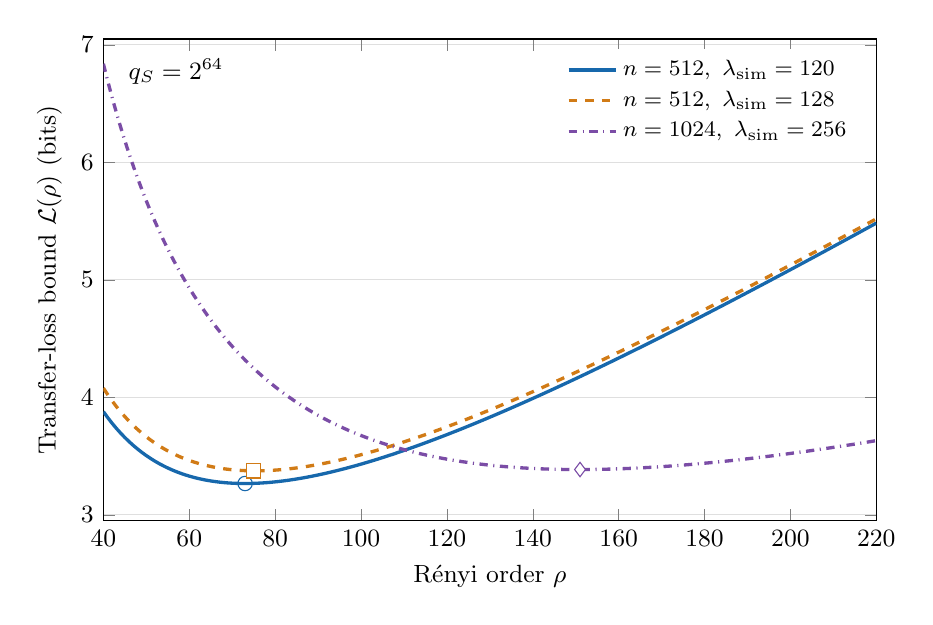
\begin{tikzpicture}
\begin{axis}[width=0.94\linewidth,height=7.7cm,
 xmin=40,xmax=220,ymin=2.95,ymax=7.05,
 xlabel={R\'enyi order $\rho$},ylabel={Transfer-loss bound $\mathcal L(\rho)$ (bits)},
 xtick={40,60,80,100,120,140,160,180,200,220},ytick={3,4,5,6,7},
 tick label style={font=\small},label style={font=\small},
 grid=major,xmajorgrids=false,grid style={gray!25},
 legend style={font=\footnotesize,draw=none,fill=white,at={(.98,.98)},anchor=north east},
 legend cell align={left},clip=true]
\addplot[color=curveone,solid,line width=1.2pt,no marks] coordinates {
(40,3.879400495183517) (41,3.828778504982262) (42,3.781640835882059) (43,3.737744395751029) (44,3.696868191742016) (45,3.6588108748165) (46,3.623388604548011) (47,3.590433186503825) (48,3.559790442453947) (49,3.531318780146347) (50,3.504887934709157) (51,3.480377858123209) (52,3.457677736832352) (53,3.436685120567694) (54,3.417305147969153) (55,3.399449856684654) (56,3.383037567387276) (57,3.367992332632689) (58,3.354243442731351) (59,3.341724981870974) (60,3.330375428626765) (61,3.320137295765718) (62,3.310956804908575) (63,3.30278359217635) (64,3.295570441432495) (65,3.289273042148869) (66,3.283849769283887) (67,3.279261482873077) (68,3.275471345302817) (69,3.272444654473325) (70,3.270148691261949) (71,3.268552579876893) (72,3.267627159848131) (73,3.267344868539612) (74,3.267679633187506) (75,3.268606771575391) (76,3.270102900550867) (77,3.272145851670754) (78,3.274714593335113) (79,3.277789158835142) (80,3.281350579797484) (81,3.285380824558576) (82,3.289862741048203) (83,3.294780003801947) (84,3.300117064758457) (85,3.30585910752986) (86,3.311992004862605) (87,3.318502279032042) (88,3.325377064937369) (89,3.332604075684566) (90,3.34017157046379) (91,3.348068324544756) (92,3.356283601228931) (93,3.36480712561127) (94,3.373629060016731) (95,3.382739980988171) (96,3.392130857712494) (97,3.401793031781271) (98,3.411718198190502) (99,3.421898387491903) (100,3.432325949015123) (101,3.442993535086661) (102,3.453894086177073) (103,3.465020816913403) (104,3.476367202898576) (105,3.487926968283983) (106,3.499694074045487) (107,3.511662706916869) (108,3.523827268938065) (109,3.536182367578739) (110,3.548722806400572) (111,3.561443576224281) (112,3.574339846769848) (113,3.587406958740618) (114,3.60064041632403) (115,3.614035880083615) (116,3.627589160218645) (117,3.641296210169444) (118,3.655153120547852) (119,3.669156113373715) (120,3.683301536599553) (121,3.697585858906728) (122,3.712005664757545) (123,3.726557649688706) (124,3.741238615832502) (125,3.756045467652995) (126,3.770975207885229) (127,3.786024933666297) (128,3.801191832847755) (129,3.816473180479567) (130,3.83186633545631) (131,3.847368737317004) (132,3.8629779031904) (133,3.878691424878065) (134,3.894506966068091) (135,3.910422259672626) (136,3.926435105282874) (137,3.942543366735552) (138,3.958744969785157) (139,3.975037899876701) (140,3.991420200013915) (141,4.007889968718154) (142,4.024445358073553) (143,4.041084571854202) (144,4.057805863729357) (145,4.074607535542916) (146,4.091487935663602) (147,4.10844545740249) (148,4.125478537494677) (149,4.142585654642106) (150,4.159765328114669) (151,4.177016116406898) (152,4.194336615947681) (153,4.211725459860575) (154,4.229181316772424) (155,4.246702889668088) (156,4.264288914789228) (157,4.281938160575171) (158,4.299649426643995) (159,4.317421542812068) (160,4.335253368150347) (161,4.353143790075857) (162,4.371091723476805) (163,4.389096109869911) (164,4.407155916588561) (165,4.425270136000485) (166,4.443437784753709) (167,4.461657903049599) (168,4.479929553941874) (169,4.498251822660494) (170,4.516623815959422) (171,4.535044661487266) (172,4.553513507179878) (173,4.572029520674014) (174,4.590591888741219) (175,4.609199816741119) (176,4.627852528093346) (177,4.646549263767376) (178,4.665289281789549) (179,4.684071856766625) (180,4.702896279425211) (181,4.721761856166469) (182,4.74066790863549) (183,4.759613773304795) (184,4.77859880107142) (185,4.797622356867056) (186,4.816683819280782) (187,4.835782580193886) (188,4.854918044426356) (189,4.874089629394581) (190,4.893296764779872) (191,4.912538892207384) (192,4.931815464935085) (193,4.951125947552383) (194,4.970469815688082) (195,4.989846555727318) (196,5.009255664537165) (197,5.028696649200594) (198,5.048169026758495) (199,5.067672323959481) (200,5.087206077017197) (201,5.106769831374862) (202,5.126363141476824) (203,5.145985570546851) (204,5.165636690372954) (205,5.185316081098502) (206,5.205023331019414) (207,5.224758036387253) (208,5.244519801217969) (209,5.264308237106158) (210,5.284122963044613) (211,5.303963605249017) (212,5.323829796987584) (213,5.343721178415512) (214,5.363637396414072) (215,5.383578104434186) (216,5.40354296234435) (217,5.423531636282768) (218,5.44354379851355) (219,5.463579127286849) (220,5.483637306702817)
};
\addlegendentry{$n=512,\ \lambda_{\mathrm{sim}}=120$}
\addplot[color=curveone,only marks,mark=o,mark options={fill=white},mark size=2.6pt,forget plot] coordinates {(73,3.267344868539612)};
\addplot[color=curvetwo,dashed,line width=1.2pt,no marks] coordinates {
(40,4.079400495183517) (41,4.023900456201774) (42,3.972117026358249) (43,3.923790907378936) (44,3.878686373560198) (45,3.836588652594278) (46,3.797301648026272) (47,3.760645952461271) (48,3.726457109120614) (49,3.694584086268796) (50,3.664887934709157) (51,3.637240603221248) (52,3.611523890678506) (53,3.587628516794109) (54,3.565453296117301) (55,3.544904402139199) (56,3.525894710244418) (57,3.508343209825672) (58,3.492174477214109) (59,3.477318202209958) (60,3.463708761960098) (61,3.451284836749325) (62,3.439989062973091) (63,3.429767719160477) (64,3.420570441432495) (65,3.412349965225792) (66,3.405061890496009) (67,3.398664467947703) (68,3.393118404126346) (69,3.388386683458832) (70,3.384434405547663) (71,3.381228636214921) (72,3.378738270959242) (73,3.376933909635502) (74,3.375787741295614) (75,3.375273438242057) (76,3.375366058445604) (77,3.376041955566858) (78,3.377278695899216) (79,3.379054981619952) (80,3.381350579797484) (81,3.384146256657341) (82,3.387423716657959) (83,3.391165545970622) (84,3.395355159996552) (85,3.399976754588683) (86,3.405015260676559) (87,3.410456302020548) (88,3.41628615584646) (89,3.422491716134004) (90,3.429060459352678) (91,3.435980412456844) (92,3.443240122968061) (93,3.450828630987615) (94,3.458735442995455) (95,3.46695050730396) (96,3.475464191045827) (97,3.484267258585395) (98,3.493350851251726) (99,3.502706468299984) (100,3.512325949015123) (101,3.52220145587874) (102,3.532325458726093) (103,3.542690719826024) (104,3.553290279821653) (105,3.564117444474459) (106,3.575165772158695) (107,3.586429062057056) (108,3.597901343012138) (109,3.609576862991583) (110,3.621450079127845) (111,3.633515648296354) (112,3.64576841819842) (113,3.658203418917609) (114,3.670815854920521) (115,3.68360109747492) (116,3.696554677460024) (117,3.709672278545513) (118,3.722949730717343) (119,3.736383004130017) (120,3.749968203266219) (121,3.763701561386067) (122,3.777579435249349) (123,3.79159830009521) (124,3.80575474486476) (125,3.820045467652995) (126,3.834467271377293) (127,3.849017059650549) (128,3.863691832847755) (129,3.878488684355536) (130,3.893404796994771) (131,3.908437439607081) (132,3.923583963796461) (133,3.938841800817915) (134,3.954208458605404) (135,3.969681518931885) (136,3.985258634694638) (137,4.000937527319494) (138,4.01671598427791) (139,4.032591856711234) (140,4.048563057156772) (141,4.064627557370637) (142,4.080783386242567) (143,4.097028627798258) (144,4.113361419284912) (145,4.129779949336019) (146,4.146282456211548) (147,4.162867226109973) (148,4.179532591548731) (149,4.196276929809891) (150,4.213098661448003) (151,4.22999624885723) (152,4.246968194895049) (153,4.264013041559921) (154,4.281129368720475) (155,4.298315792893894) (156,4.315570966071279) (157,4.33289357458791) (158,4.3502823380364) (159,4.367736008220873) (160,4.385253368150347) (161,4.402833231069645) (162,4.420474439526187) (163,4.438175864471138) (164,4.455936404393439) (165,4.473754984485334) (166,4.491630555838046) (167,4.509562094666366) (168,4.527548601560921) (169,4.545589100767002) (170,4.563682639488833) (171,4.581828287218261) (172,4.600025135086855) (173,4.618272295240488) (174,4.636568900235472) (175,4.654914102455404) (176,4.673307073547892) (177,4.69174700388037) (178,4.710233102014269) (179,4.728764594196792) (180,4.747340723869655) (181,4.765960751194093) (182,4.784623952591534) (183,4.803329620299331) (184,4.822077061940985) (185,4.8408656001103) (186,4.859694571968954) (187,4.878563328856988) (188,4.897471235915718) (189,4.916417671722623) (190,4.935402027937767) (191,4.954423708961311) (192,4.973482131601751) (193,4.992576724754456) (194,5.011706929090145) (195,5.03087219675296) (196,5.050071991067778) (197,5.069305786256431) (198,5.088573067162535) (199,5.107873328984607) (200,5.127206077017197) (201,5.146570826399738) (202,5.165967101872863) (203,5.185394437541925) (204,5.204852376647464) (205,5.224340471342404) (206,5.243858282475725) (207,5.263405379382422) (208,5.282981339679507) (209,5.302585749067879) (210,5.322218201139852) (211,5.341878297192145) (212,5.361565646044188) (213,5.381279863861522) (214,5.401020573984166) (215,5.420787406759767) (216,5.440579999381386) (217,5.460397995729773) (218,5.480241046219972) (219,5.500108807652146) (220,5.520000943066453)
};
\addlegendentry{$n=512,\ \lambda_{\mathrm{sim}}=128$}
\addplot[color=curvetwo,only marks,mark=square*,mark options={fill=white},mark size=2.6pt,forget plot] coordinates {(75,3.375273438242057)};
\addplot[color=curvethree,dashdotted,line width=1.2pt,no marks] coordinates {
(40,6.839624805407581) (41,6.694799675353113) (42,6.557407762488621) (43,6.426930470266016) (44,6.30289634727794) (45,6.184875848908804) (46,6.072476782248717) (47,5.965340332507784) (48,5.8631375861286) (49,5.765566479640078) (50,5.672349114648815) (51,5.583229388713839) (52,5.497970899581938) (53,5.416355086679393) (54,5.338179579104607) (55,5.26325672383974) (56,5.191412271653939) (57,5.122484201332551) (58,5.056321665537796) (59,4.992784043870047) (60,4.93174009062299) (61,4.873067166366129) (62,4.816650543890294) (63,4.762382780253562) (64,4.710163147697882) (65,4.659897117096468) (66,4.611495888360517) (67,4.56487596289907) (68,4.519958753802986) (69,4.476670229925975) (70,4.43494059047296) (71,4.394703967088027) (72,4.355898150768367) (73,4.318464341223653) (74,4.282346916557631) (75,4.247493221375179) (76,4.213853371617761) (77,4.181380074606506) (78,4.150028462928126) (79,4.119755940937092) (80,4.090522042770155) (81,4.0622883008783) (82,4.035018124178314) (83,4.008676685012685) (84,3.983230814183781) (85,3.958648903397387) (86,3.93490081451251) (87,3.911957795049809) (88,3.889792399460823) (89,3.868378415704889) (90,3.847690796720925) (91,3.827705596417572) (92,3.808399909837873) (93,3.789751817184313) (94,3.771740331416716) (95,3.754345349159759) (96,3.737547604678753) (97,3.7213286267023) (98,3.705670697888441) (99,3.690556816747423) (100,3.675970661849079) (101,3.661896558156518) (102,3.648319445340178) (103,3.635224847937665) (104,3.622598847235136) (105,3.610428054755468) (106,3.59869958724709) (107,3.587401043075311) (108,3.576520479925244) (109,3.566046393732089) (110,3.555967698760677) (111,3.546273708761788) (112,3.536954119137962) (113,3.527998990056251) (114,3.519398730449773) (115,3.511144082853976) (116,3.50322610902722) (117,3.495636176308779) (118,3.488365944670491) (119,3.481407354421276) (120,3.474752614526426) (121,3.468394191506095) (122,3.462324798879779) (123,3.456537387125688) (124,3.451025134125964) (125,3.445781436070516) (126,3.440799898794021) (127,3.436074329522188) (128,3.431598729004923) (129,3.427367284015392) (130,3.423374360195277) (131,3.419614495227737) (132,3.416082392320683) (133,3.412772913984044) (134,3.40968107608566) (135,3.406802042171365) (136,3.404131118035639) (137,3.401663746530062) (138,3.399395502597473) (139,3.397322088520481) (140,3.395439329373625) (141,3.393743168669042) (142,3.392229664186137) (143,3.390894983976216) (144,3.389735402533606) (145,3.388747297125203) (146,3.387927144270867) (147,3.387271516367466) (148,3.386777078449793) (149,3.386440585081906) (150,3.386258877372824) (151,3.386228880110794) (152,3.386347599010691) (153,3.386612118069353) (154,3.38701959702396) (155,3.387567268908796) (156,3.388252437705985) (157,3.389072476086005) (158,3.390024823234004) (159,3.391106982758146) (160,3.392316520676391) (161,3.393651063478301) (162,3.395108296258637) (163,3.396685960919648) (164,3.398381854439138) (165,3.400193827201511) (166,3.402119781389137) (167,3.404157669431513) (168,3.406305492509818) (169,3.408561299114548) (170,3.410923183654073) (171,3.413389285112005) (172,3.415957785751406) (173,3.418626909863939) (174,3.421394922562147) (175,3.424260128613145) (176,3.427220871312066) (177,3.430275531393702) (178,3.433422525980829) (179,3.436660307567778) (180,3.439987363037897) (181,3.443402212713576) (182,3.44690340943759) (183,3.450489537684569) (184,3.45415921270143) (185,3.4579110796757) (186,3.461743812930659) (187,3.465656115146304) (188,3.469646716605189) (189,3.473714374462193) (190,3.477857872037358) (191,3.482076018130931) (192,3.486367646359823) (193,3.490731614514686) (194,3.495166803936883) (195,3.499672118914617) (196,3.50424648609756) (197,3.508888853929297) (198,3.513598192096977) (199,3.518373490997556) (200,3.52321376122005) (201,3.528118033043248) (202,3.533085355948335) (203,3.538114798145935) (204,3.54320544611705) (205,3.548356404167443) (206,3.553566793994997) (207,3.55883575426962) (208,3.564162440225257) (209,3.569546023263625) (210,3.574985690569266) (211,3.580480644735546) (212,3.58603010340124) (213,3.591633298897349) (214,3.597289477903832) (215,3.602997901115902) (216,3.608757842919601) (217,3.614568591076344) (218,3.620429446416145) (219,3.626339722539245) (220,3.63229874552588)
};
\addlegendentry{$n=1024,\ \lambda_{\mathrm{sim}}=256$}
\addplot[color=curvethree,only marks,mark=diamond*,mark options={fill=white},mark size=2.6pt,forget plot] coordinates {(151,3.386228880110794)};
\node[anchor=north west,font=\small] at (rel axis cs:.02,.98) {$q_S=2^{64}$};
\end{axis}
\end{tikzpicture}
\caption{The same analytic transfer expressions for the three simulator-probability inputs. Markers indicate the orders $73$, $75$ and $151$ used for the certified bounds. The curves draw numerical values of upper-bound expressions; the oracle and hardness costs enter the security theorem separately.}
\label{fig:transfer}
\end{figure}

The other costs remain visible. At $q_S=2^{64}$ and $\kappa=320$, the
classical programming expression is approximately $2^{-191.415}$ for
$q_H=2^{64}$ and $2^{-128}$ for $q_H=2^{128}$. The conservative quantum
expression is instead approximately $2^{-62.915}$ and $2^{-31.415}$.
These additive probability terms enter alongside the quantum extraction
loss and simulation work. Their size makes the classical theorem the
principal concrete-security application at these query budgets.

Finally, an optional real signer capped at $\ell$ norm attempts per query
adds at most $q_S(bD_0)^\ell$ to either theorem. At $q_S\le2^{64}$,
$\ell=32$ for degree 512 and $\ell=16$ for degree 1024 give a bound below
$2^{-390}$. This bounds the real signer's attempt limit; \eqref{eq:finite-pool}
bounds exhaustion of the simulator's separate public pool.


\section{What the complete argument tells us}

The proof connects two experiments on the same public equation. The signer chooses a target and samples an accepted preimage; the public simulator chooses an accepted vector and computes its target. The norm cutoff introduces target-dependent acceptance weights, so ordinary Gaussian smoothing must be supplemented by control of the rejected image.

The key-quality bound controls dual-lattice Gaussian masses. The exact integer-tail contour separates zero, parity, and remaining rational-angle contributions. Merging the character classes avoids a factor equal to the number of syndromes. Certified evaluation then bounds the acceptance variance and accepted-image chi-square distance for every permitted key.

The security argument preserves these small errors through conditioning and interaction. The conditional-excess lemma handles the sampler; the density floor supplies the reverse target moment. Comparing target and preimage jointly gives one event-probability exponent, and a common procedure consumes independent pairs even when messages are chosen adaptively.

Fresh salts and a finite public Gaussian pool complete the simulation, with an explicit programming error, sampling-call budget, and pool-failure bound. Unprogrammed-input forgeries yield the uniform-target problem; strong forgeries additionally use the distinct-preimage game and canonical representation. The quantum-oracle corollary retains its programming, extraction, and simulation costs.

\subsection{How to interpret the quantitative result}

There are several different quantities in this chain, and their units matter. The variance is a squared-average variation in acceptance probability over uniform targets. The chi-square distance is a squared density discrepancy of the accepted public image. Both are dimensionless. The transfer loss is a base-two logarithmic loss in a conditional forgery-probability bound, measured in bits. Signing and hash queries are counts of oracle interactions. The Gaussian-pool budget counts sampler calls, while the reduction's local operations contribute actual work. None of these quantities can replace the others in the final theorem.

The analytic theorem is uniform over keys meeting its geometric hypotheses. The cryptographic assumptions measure hardness on the specified trapdoor-generated key distribution, at the solver resources charged in the reduction.

\subsection{The model boundary is part of the result}
\label{sec:model-boundary}

The covered signer draws one independent salt after each chosen message, keeps its target fixed during private norm retries, uses a sampler with the declared distributional profile, and returns only the final specified output. The concrete sampler application is exact arithmetic. The proof covers the mathematical signature and the stated canonical compressed wrapper with adequate buffers and public encoding errors.

A finite-precision signer requires a profile for its actual sampling errors. Rejection on a total padded encoding budget introduces another conditioning event. Caller-selected or reused salts change the fresh-input analysis. Exposed retry counts or timing provide a different observation to the adversary. Several keys or an aggregate interface require corresponding key and oracle models.

\clearpage
\appendix
\section{Notation at a glance}

The table collects the recurring objects. Gaussian exponents and probability-comparison orders use different symbols because they perform different jobs.

\begin{longtable}{@{}p{0.23\textwidth}p{0.73\textwidth}@{}}
\toprule
Symbol & Meaning \\
\midrule
\endhead
$n$, $d=2n$ & Polynomial degree and dimension of the integer coefficient vector. \\
$q=12289$ & Modulus in the public syndrome equation. \\
$F_h$, $\Lambda_h$ & Public map $(u,v)\mapsto u+hv\bmod q$, and its kernel lattice. \\
$Y$, $N=|Y|$ & Syndrome quotient and its cardinality $q^n$. \\
$U$ & Uniform probability law on the finite quotient. \\
$\sigma$, $\alpha$ & Gaussian width and exponent parameter $\alpha=1/(2\sigma^2)$. \\
$B_0$ & Upper bound $(117/100)\sqrt q$ on Gram--Schmidt lengths. \\
$\eps_{\mathrm{des}}$, $\xi$ & Sampler-width design parameter and the separate tuning parameter in the Gaussian-mass inequalities. \\
$\rho_c(S)$ & Unnormalized Gaussian mass $\sum_{x\in S}e^{-c\norm{x}^2}$, for $c>0$. \\
$G$, $G_y$ & Ambient integer Gaussian and that Gaussian conditioned on syndrome $y$. \\
$P_y$ & Actual exact-arithmetic preimage-sampler law under the declared contract. \\
$T$, $K=T+1$ & Largest accepted squared norm and first rejected integer squared norm. \\
$A$ & Event $\norm{z}^2\le T$. \\
$a_y$ & Exact coset-Gaussian acceptance probability $G_y(A)$. \\
$p(y)$, $r(y)$ & Unconditioned and rejected ambient-image densities relative to $U$. \\
$\delta$ & Ambient rejection probability $\E_U r$; not generally the uniform-coset mean rejection probability. \\
$Q_0$, $R$ & Centered image and tail density norms $\norm{p-1}_{L^2(U)}$ and $\norm{r-\delta}_{L^2(U)}$. \\
$D_0$ & Uniform upper bound on rejection probability in any coset. \\
$\nu$, $w(y)$ & Accepted ambient syndrome law and its density $w=\mathrm d\nu/\mathrm dU$. \\
$\rho>1$, $M_\rho$ & Order and unrooted likelihood-ratio moment used in the security comparison. \\
$L$, $M$ & Joint target/preimage laws for fixed uniform-target signing and public accepted-Gaussian simulation. \\
$I_t$, $S_C$ & Success probabilities in the stated uniform-target and unconditioned Gaussian distinct-preimage games, with the indicated challenge budgets. \\
$q_S$, $q_H$, $\kappa$ & Signing queries, hash queries, and salt length in bits. \\
$C$, $\eps_{\mathrm{pool}}$ & Finite Gaussian-pool size and upper bound on its failure probability. \\
$Q=q_H+q_S+1$ & Background-oracle query budget in the stated quantum reduction. \\
\bottomrule
\end{longtable}

\end{document}
